\documentclass[1p]{elsarticle_modified}
%\bibliographystyle{elsarticle-num}

%\usepackage[colorlinks]{hyperref}
%\usepackage{abbrmath_seonhwa} %\Abb, \Ascr, \Acal ,\Abf, \Afrak
\usepackage{amsfonts}
\usepackage{amssymb}
\usepackage{amsmath}
\usepackage{amsthm}
\usepackage{scalefnt}
\usepackage{amsbsy}
\usepackage{kotex}
\usepackage{caption}
\usepackage{subfig}
\usepackage{color}
\usepackage{graphicx}
\usepackage{xcolor} %% white, black, red, green, blue, cyan, magenta, yellow
\usepackage{float}
\usepackage{setspace}
\usepackage{hyperref}

\usepackage{tikz}
\usetikzlibrary{arrows}

\usepackage{multirow}
\usepackage{array} % fixed length table
\usepackage{hhline}

%%%%%%%%%%%%%%%%%%%%%
\makeatletter
\renewcommand*\env@matrix[1][\arraystretch]{%
	\edef\arraystretch{#1}%
	\hskip -\arraycolsep
	\let\@ifnextchar\new@ifnextchar
	\array{*\c@MaxMatrixCols c}}
\makeatother %https://tex.stackexchange.com/questions/14071/how-can-i-increase-the-line-spacing-in-a-matrix
%%%%%%%%%%%%%%%

\usepackage[normalem]{ulem}

\newcommand{\msout}[1]{\ifmmode\text{\sout{\ensuremath{#1}}}\else\sout{#1}\fi}
%SOURCE: \msout is \stkout macro in https://tex.stackexchange.com/questions/20609/strikeout-in-math-mode

\newcommand{\cancel}[1]{
	\ifmmode
	{\color{red}\msout{#1}}
	\else
	{\color{red}\sout{#1}}
	\fi
}

\newcommand{\add}[1]{
	{\color{blue}\uwave{#1}}
}

\newcommand{\replace}[2]{
	\ifmmode
	{\color{red}\msout{#1}}{\color{blue}\uwave{#2}}
	\else
	{\color{red}\sout{#1}}{\color{blue}\uwave{#2}}
	\fi
}

\newcommand{\Sol}{\mathcal{S}} %segment
\newcommand{\D}{D} %diagram
\newcommand{\A}{\mathcal{A}} %arc


%%%%%%%%%%%%%%%%%%%%%%%%%%%%%5 test

\def\sl{\operatorname{\textup{SL}}(2,\Cbb)}
\def\psl{\operatorname{\textup{PSL}}(2,\Cbb)}
\def\quan{\mkern 1mu \triangleright \mkern 1mu}

\theoremstyle{definition}
\newtheorem{thm}{Theorem}[section]
\newtheorem{prop}[thm]{Proposition}
\newtheorem{lem}[thm]{Lemma}
\newtheorem{ques}[thm]{Question}
\newtheorem{cor}[thm]{Corollary}
\newtheorem{defn}[thm]{Definition}
\newtheorem{exam}[thm]{Example}
\newtheorem{rmk}[thm]{Remark}
\newtheorem{alg}[thm]{Algorithm}

\newcommand{\I}{\sqrt{-1}}
\begin{document}

%\begin{frontmatter}
%
%\title{Boundary parabolic representations of knots up to 8 crossings}
%
%%% Group authors per affiliation:
%\author{Yunhi Cho} 
%\address{Department of Mathematics, University of Seoul, Seoul, Korea}
%\ead{yhcho@uos.ac.kr}
%
%
%\author{Seonhwa Kim} %\fnref{s_kim}}
%\address{Center for Geometry and Physics, Institute for Basic Science, Pohang, 37673, Korea}
%\ead{ryeona17@ibs.re.kr}
%
%\author{Hyuk Kim}
%\address{Department of Mathematical Sciences, Seoul National University, Seoul 08826, Korea}
%\ead{hyukkim@snu.ac.kr}
%
%\author{Seokbeom Yoon}
%\address{Department of Mathematical Sciences, Seoul National University, Seoul, 08826,  Korea}
%\ead{sbyoon15@snu.ac.kr}
%
%\begin{abstract}
%We find all boundary parabolic representation of knots up to 8 crossings.
%
%\end{abstract}
%\begin{keyword}
%    \MSC[2010] 57M25 
%\end{keyword}
%
%\end{frontmatter}

%\linenumbers
%\tableofcontents
%
\newcommand\colored[1]{\textcolor{white}{\rule[-0.35ex]{0.8em}{1.4ex}}\kern-0.8em\color{red} #1}%
%\newcommand\colored[1]{\textcolor{white}{ #1}\kern-2.17ex	\textcolor{white}{ #1}\kern-1.81ex	\textcolor{white}{ #1}\kern-2.15ex\color{red}#1	}

{\Large $\underline{12n_{0857}~(K12n_{0857})}$}

\setlength{\tabcolsep}{10pt}
\renewcommand{\arraystretch}{1.6}
\vspace{1cm}\begin{tabular}{m{100pt}>{\centering\arraybackslash}m{274pt}}
\multirow{5}{120pt}{
	\centering
	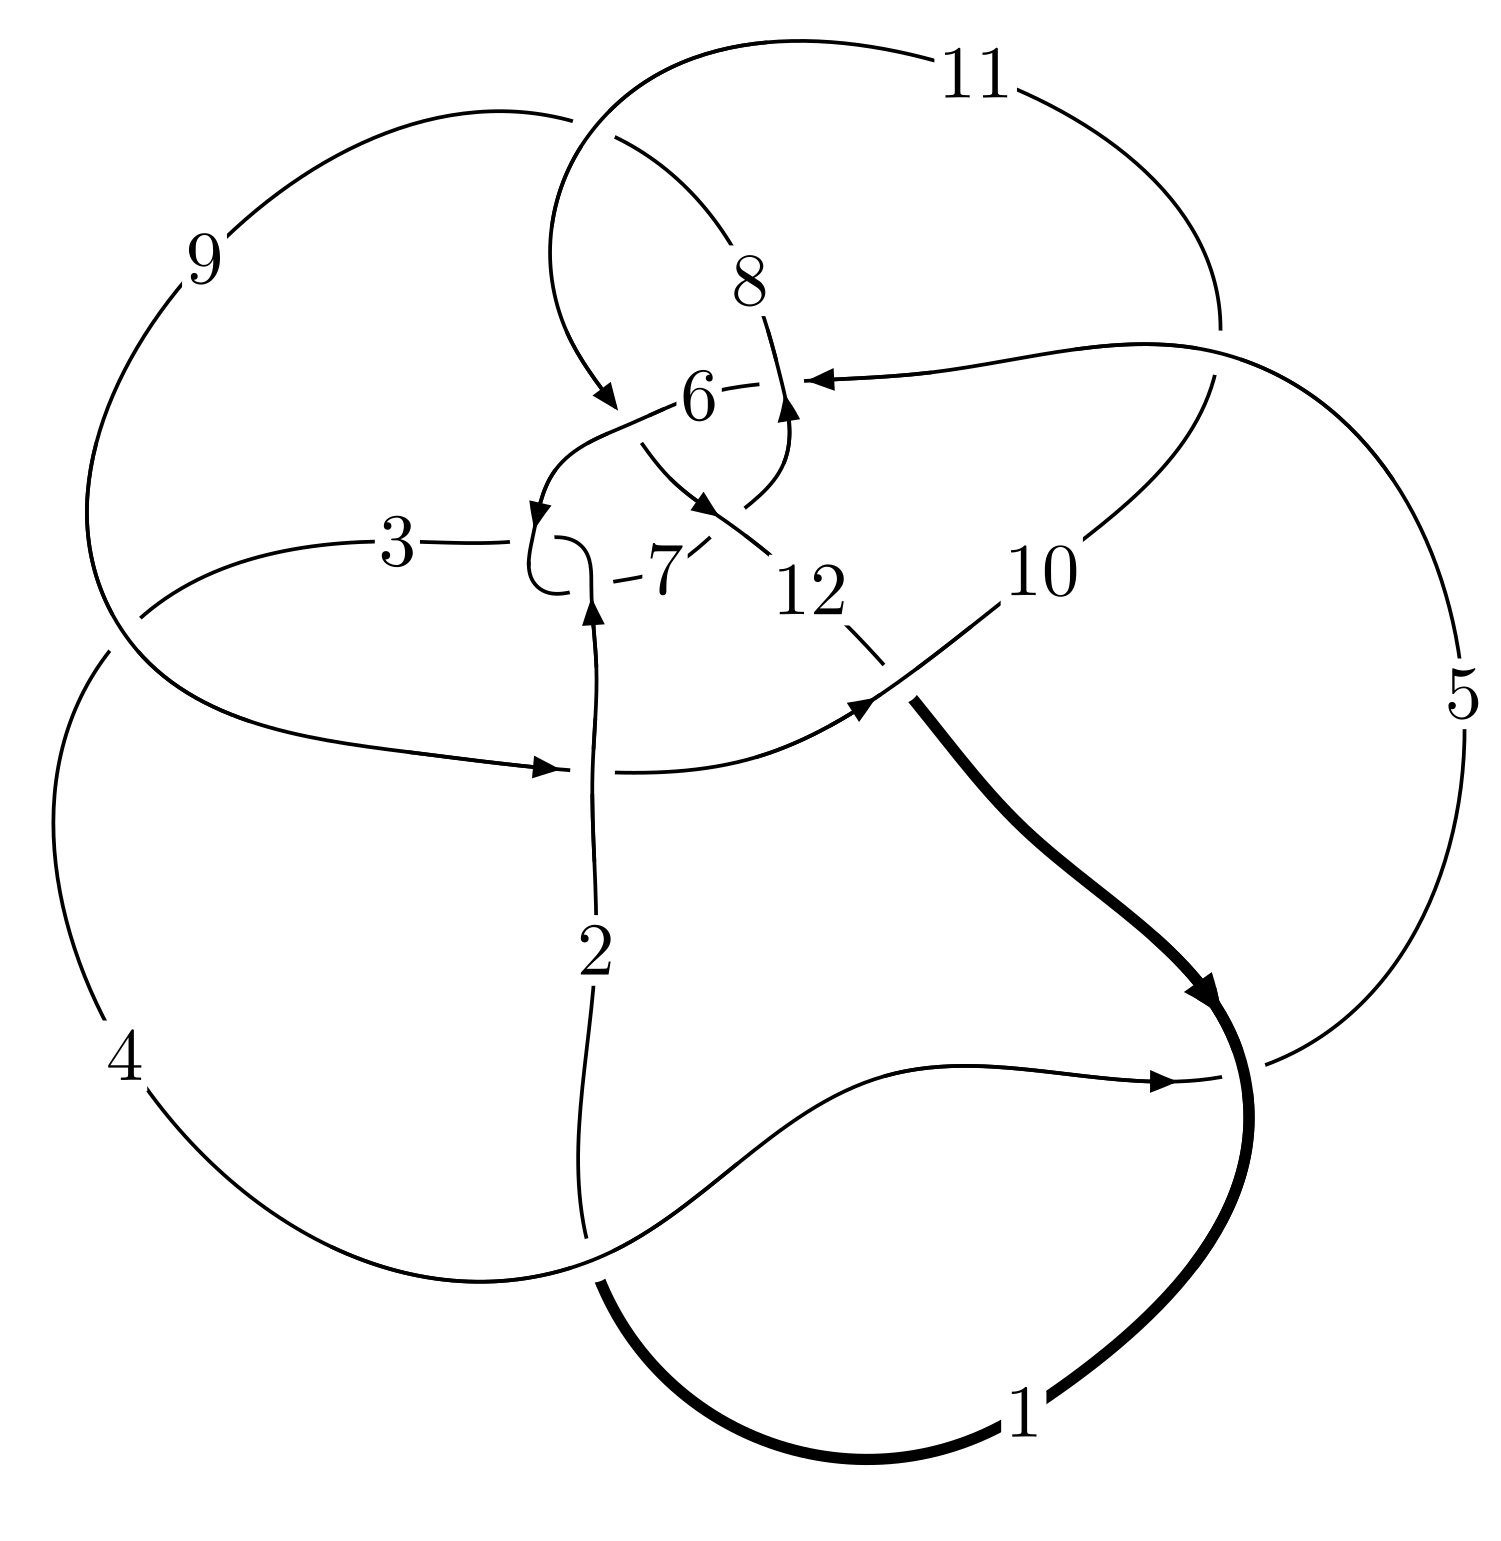
\includegraphics[width=112pt]{../../../GIT/diagram.site/Diagrams/png/2946_12n_0857.png}\\
\ \ \ A knot diagram\footnotemark}&
\allowdisplaybreaks
\textbf{Linearized knot diagam} \\
\cline{2-2}
 &
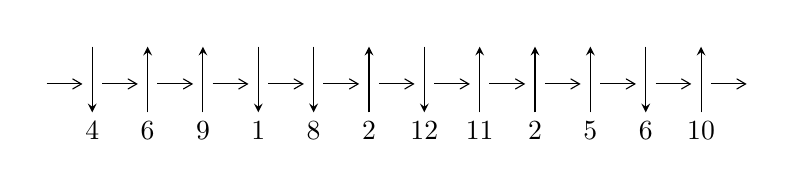
\begin{tikzpicture}[x=20pt, y=17pt]
	% nodes
	\node (C0) at (0, 0) {};
	\node (C1) at (1, 0) {};
	\node (C1U) at (1, +1) {};
	\node (C1D) at (1, -1) {4};

	\node (C2) at (2, 0) {};
	\node (C2U) at (2, +1) {};
	\node (C2D) at (2, -1) {6};

	\node (C3) at (3, 0) {};
	\node (C3U) at (3, +1) {};
	\node (C3D) at (3, -1) {9};

	\node (C4) at (4, 0) {};
	\node (C4U) at (4, +1) {};
	\node (C4D) at (4, -1) {1};

	\node (C5) at (5, 0) {};
	\node (C5U) at (5, +1) {};
	\node (C5D) at (5, -1) {8};

	\node (C6) at (6, 0) {};
	\node (C6U) at (6, +1) {};
	\node (C6D) at (6, -1) {2};

	\node (C7) at (7, 0) {};
	\node (C7U) at (7, +1) {};
	\node (C7D) at (7, -1) {12};

	\node (C8) at (8, 0) {};
	\node (C8U) at (8, +1) {};
	\node (C8D) at (8, -1) {11};

	\node (C9) at (9, 0) {};
	\node (C9U) at (9, +1) {};
	\node (C9D) at (9, -1) {2};

	\node (C10) at (10, 0) {};
	\node (C10U) at (10, +1) {};
	\node (C10D) at (10, -1) {5};

	\node (C11) at (11, 0) {};
	\node (C11U) at (11, +1) {};
	\node (C11D) at (11, -1) {6};

	\node (C12) at (12, 0) {};
	\node (C12U) at (12, +1) {};
	\node (C12D) at (12, -1) {10};
	\node (C13) at (13, 0) {};

	% arrows
	\draw[->,>={angle 60}]
	(C0) edge (C1) (C1) edge (C2) (C2) edge (C3) (C3) edge (C4) (C4) edge (C5) (C5) edge (C6) (C6) edge (C7) (C7) edge (C8) (C8) edge (C9) (C9) edge (C10) (C10) edge (C11) (C11) edge (C12) (C12) edge (C13) ;	\draw[->,>=stealth]
	(C1U) edge (C1D) (C2D) edge (C2U) (C3D) edge (C3U) (C4U) edge (C4D) (C5U) edge (C5D) (C6D) edge (C6U) (C7U) edge (C7D) (C8D) edge (C8U) (C9D) edge (C9U) (C10D) edge (C10U) (C11U) edge (C11D) (C12D) edge (C12U) ;
	\end{tikzpicture} \\
\hhline{~~} \\& 
\textbf{Solving Sequence} \\ \cline{2-2} 
 &
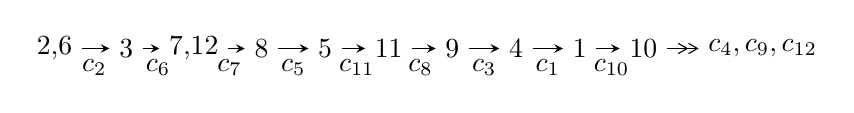
\begin{tikzpicture}[x=23pt, y=7pt]
	% node
	\node (A0) at (-1/8, 0) {2,6};
	\node (A1) at (1, 0) {3};
	\node (A2) at (33/16, 0) {7,12};
	\node (A3) at (25/8, 0) {8};
	\node (A4) at (33/8, 0) {5};
	\node (A5) at (41/8, 0) {11};
	\node (A6) at (49/8, 0) {9};
	\node (A7) at (57/8, 0) {4};
	\node (A8) at (65/8, 0) {1};
	\node (A9) at (73/8, 0) {10};
	\node (C1) at (1/2, -1) {$c_{2}$};
	\node (C2) at (3/2, -1) {$c_{6}$};
	\node (C3) at (21/8, -1) {$c_{7}$};
	\node (C4) at (29/8, -1) {$c_{5}$};
	\node (C5) at (37/8, -1) {$c_{11}$};
	\node (C6) at (45/8, -1) {$c_{8}$};
	\node (C7) at (53/8, -1) {$c_{3}$};
	\node (C8) at (61/8, -1) {$c_{1}$};
	\node (C9) at (69/8, -1) {$c_{10}$};
	\node (A10) at (11, 0) {$c_{4},c_{9},c_{12}$};

	% edge
	\draw[->,>=stealth]	
	(A0) edge (A1) (A1) edge (A2) (A2) edge (A3) (A3) edge (A4) (A4) edge (A5) (A5) edge (A6) (A6) edge (A7) (A7) edge (A8) (A8) edge (A9) ;
	\draw[->>,>={angle 60}]	
	(A9) edge (A10);
\end{tikzpicture} \\ 

\end{tabular} \\

\footnotetext{
The image of knot diagram is generated by the software ``\textbf{Draw programme}" developed by Andrew Bartholomew(\url{http://www.layer8.co.uk/maths/draw/index.htm\#Running-draw}), where we modified some parts for our purpose(\url{https://github.com/CATsTAILs/LinksPainter}).
}\phantom \\ \newline 
\centering \textbf{Ideals for irreducible components\footnotemark of $X_{\text{par}}$} 
 
\begin{align*}
I^u_{1}&=\langle 
-2.54221\times10^{715} u^{109}+1.88993\times10^{715} u^{108}+\cdots+2.43228\times10^{719} b-1.89889\times10^{720},\\
\phantom{I^u_{1}}&\phantom{= \langle  }-5.21983\times10^{720} u^{109}+3.53329\times10^{720} u^{108}+\cdots+2.79846\times10^{724} a-6.69018\times10^{725},\\
\phantom{I^u_{1}}&\phantom{= \langle  }u^{110}- u^{109}+\cdots+158844 u-23011\rangle \\
I^u_{2}&=\langle 
-1.69300\times10^{47} u^{40}+1.74572\times10^{46} u^{39}+\cdots+3.46916\times10^{46} b-4.11027\times10^{46},\\
\phantom{I^u_{2}}&\phantom{= \langle  }-1.42407\times10^{47} u^{40}+2.07337\times10^{46} u^{39}+\cdots+3.46916\times10^{46} a-2.12701\times10^{46},\;u^{41}-6 u^{39}+\cdots+u-1\rangle \\
\\
\end{align*}
\raggedright * 2 irreducible components of $\dim_{\mathbb{C}}=0$, with total 151 representations.\\
\footnotetext{All coefficients of polynomials are rational numbers. But the coefficients are sometimes approximated in decimal forms when there is not enough margin.}
\newpage
\renewcommand{\arraystretch}{1}
\centering \section*{I. $I^u_{1}= \langle -2.54\times10^{715} u^{109}+1.89\times10^{715} u^{108}+\cdots+2.43\times10^{719} b-1.90\times10^{720},\;-5.22\times10^{720} u^{109}+3.53\times10^{720} u^{108}+\cdots+2.80\times10^{724} a-6.69\times10^{725},\;u^{110}- u^{109}+\cdots+158844 u-23011 \rangle$}
\flushleft \textbf{(i) Arc colorings}\\
\begin{tabular}{m{7pt} m{180pt} m{7pt} m{180pt} }
\flushright $a_{2}=$&$\begin{pmatrix}1\\0\end{pmatrix}$ \\
\flushright $a_{6}=$&$\begin{pmatrix}0\\u\end{pmatrix}$ \\
\flushright $a_{3}=$&$\begin{pmatrix}1\\- u^2\end{pmatrix}$ \\
\flushright $a_{7}=$&$\begin{pmatrix}u\\u\end{pmatrix}$ \\
\flushright $a_{12}=$&$\begin{pmatrix}0.000186525 u^{109}-0.000126258 u^{108}+\cdots-86.7680 u+23.9067\\0.000104520 u^{109}-0.0000777021 u^{108}+\cdots-22.7251 u+7.80705\end{pmatrix}$ \\
\flushright $a_{8}=$&$\begin{pmatrix}0.000187611 u^{109}-0.000113060 u^{108}+\cdots-7.21058 u+4.09697\\-0.0000441421 u^{109}+0.0000112573 u^{108}+\cdots+24.8025 u-4.20354\end{pmatrix}$ \\
\flushright $a_{5}=$&$\begin{pmatrix}0.000353843 u^{109}-0.000263570 u^{108}+\cdots-154.257 u+32.4618\\0.0000988927 u^{109}-0.0000682856 u^{108}+\cdots-26.1513 u+8.57675\end{pmatrix}$ \\
\flushright $a_{11}=$&$\begin{pmatrix}0.000186525 u^{109}-0.000126258 u^{108}+\cdots-86.7680 u+23.9067\\0.000103255 u^{109}-0.0000818589 u^{108}+\cdots-17.4442 u+6.42025\end{pmatrix}$ \\
\flushright $a_{9}=$&$\begin{pmatrix}-0.000258536 u^{109}+0.000209102 u^{108}+\cdots+120.512 u-25.4063\\0.0000986832 u^{109}-0.0000625693 u^{108}+\cdots-35.6479 u+8.19303\end{pmatrix}$ \\
\flushright $a_{4}=$&$\begin{pmatrix}-0.000159884 u^{109}+0.0000964328 u^{108}+\cdots+92.8382 u-16.6342\\0.000138065 u^{109}-0.0000904983 u^{108}+\cdots-51.6830 u+12.8395\end{pmatrix}$ \\
\flushright $a_{1}=$&$\begin{pmatrix}0.0000566483 u^{109}-0.0000528472 u^{108}+\cdots+52.8264 u-5.41832\\-0.0000756289 u^{109}+0.0000417867 u^{108}+\cdots+25.4750 u-5.64856\end{pmatrix}$ \\
\flushright $a_{10}=$&$\begin{pmatrix}-0.000159853 u^{109}+0.000146533 u^{108}+\cdots+84.8642 u-17.2133\\0.0000986832 u^{109}-0.0000625693 u^{108}+\cdots-35.6479 u+8.19303\end{pmatrix}$\\&\end{tabular}
\flushleft \textbf{(ii) Obstruction class $= -1$}\\~\\
\flushleft \textbf{(iii) Cusp Shapes $= 0.000468187 u^{109}-0.000486994 u^{108}+\cdots-109.891 u+53.5401$}\\~\\
\newpage\renewcommand{\arraystretch}{1}
\flushleft \textbf{(iv) u-Polynomials at the component}\newline \\
\begin{tabular}{m{50pt}|m{274pt}}
Crossings & \hspace{64pt}u-Polynomials at each crossing \\
\hline $$\begin{aligned}c_{1},c_{4}\end{aligned}$$&$\begin{aligned}
&u^{110}-5 u^{109}+\cdots-655 u+27
\end{aligned}$\\
\hline $$\begin{aligned}c_{2},c_{6}\end{aligned}$$&$\begin{aligned}
&u^{110}- u^{109}+\cdots+158844 u-23011
\end{aligned}$\\
\hline $$\begin{aligned}c_{3}\end{aligned}$$&$\begin{aligned}
&u^{110}+u^{109}+\cdots-27299702743 u-7633881929
\end{aligned}$\\
\hline $$\begin{aligned}c_{5}\end{aligned}$$&$\begin{aligned}
&u^{110}-7 u^{109}+\cdots+32 u-1
\end{aligned}$\\
\hline $$\begin{aligned}c_{7}\end{aligned}$$&$\begin{aligned}
&u^{110}+25 u^{108}+\cdots+2741658038 u-256908883
\end{aligned}$\\
\hline $$\begin{aligned}c_{8}\end{aligned}$$&$\begin{aligned}
&u^{110}-6 u^{109}+\cdots-132 u-121
\end{aligned}$\\
\hline $$\begin{aligned}c_{9}\end{aligned}$$&$\begin{aligned}
&u^{110}-27 u^{108}+\cdots-348627733 u-55663493
\end{aligned}$\\
\hline $$\begin{aligned}c_{10}\end{aligned}$$&$\begin{aligned}
&u^{110}+4 u^{109}+\cdots+979761921 u+106831211
\end{aligned}$\\
\hline $$\begin{aligned}c_{11}\end{aligned}$$&$\begin{aligned}
&u^{110}+18 u^{108}+\cdots+1919803 u-465261
\end{aligned}$\\
\hline $$\begin{aligned}c_{12}\end{aligned}$$&$\begin{aligned}
&u^{110}-5 u^{109}+\cdots-1146282 u+43209
\end{aligned}$\\
\hline
\end{tabular}\\~\\
\newpage\renewcommand{\arraystretch}{1}
\flushleft \textbf{(v) Riley Polynomials at the component}\newline \\
\begin{tabular}{m{50pt}|m{274pt}}
Crossings & \hspace{64pt}Riley Polynomials at each crossing \\
\hline $$\begin{aligned}c_{1},c_{4}\end{aligned}$$&$\begin{aligned}
&y^{110}+77 y^{109}+\cdots+13397 y+729
\end{aligned}$\\
\hline $$\begin{aligned}c_{2},c_{6}\end{aligned}$$&$\begin{aligned}
&y^{110}-93 y^{109}+\cdots-21526553292 y+529506121
\end{aligned}$\\
\hline $$\begin{aligned}c_{3}\end{aligned}$$&$\begin{aligned}
&y^{110}-71 y^{109}+\cdots-1.44\times10^{21} y+5.83\times10^{19}
\end{aligned}$\\
\hline $$\begin{aligned}c_{5}\end{aligned}$$&$\begin{aligned}
&y^{110}-3 y^{109}+\cdots-512 y+1
\end{aligned}$\\
\hline $$\begin{aligned}c_{7}\end{aligned}$$&$\begin{aligned}
&y^{110}+50 y^{109}+\cdots+1760931224300394538 y+66002174164307689
\end{aligned}$\\
\hline $$\begin{aligned}c_{8}\end{aligned}$$&$\begin{aligned}
&y^{110}-40 y^{109}+\cdots-2526964 y+14641
\end{aligned}$\\
\hline $$\begin{aligned}c_{9}\end{aligned}$$&$\begin{aligned}
&y^{110}-54 y^{109}+\cdots-28826776772721039 y+3098424452961049
\end{aligned}$\\
\hline $$\begin{aligned}c_{10}\end{aligned}$$&$\begin{aligned}
&y^{110}-64 y^{109}+\cdots-562423846261318061 y+11412907643726521
\end{aligned}$\\
\hline $$\begin{aligned}c_{11}\end{aligned}$$&$\begin{aligned}
&y^{110}+36 y^{109}+\cdots+4003166674991 y+216467798121
\end{aligned}$\\
\hline $$\begin{aligned}c_{12}\end{aligned}$$&$\begin{aligned}
&y^{110}-47 y^{109}+\cdots-179416969920 y+1867017681
\end{aligned}$\\
\hline
\end{tabular}\\~\\
\newpage\flushleft \textbf{(vi) Complex Volumes and Cusp Shapes}
$$\begin{array}{c|c|c}  
\text{Solutions to }I^u_{1}& \I (\text{vol} + \sqrt{-1}CS) & \text{Cusp shape}\\
 \hline 
\begin{aligned}
u &= \phantom{-}0.273687 + 0.960931 I \\
a &= -0.484952 - 0.110282 I \\
b &= -0.672250 + 0.036578 I\end{aligned}
 & -1.25797 + 2.48843 I & \phantom{-0.000000 } 0 \\ \hline\begin{aligned}
u &= \phantom{-}0.273687 - 0.960931 I \\
a &= -0.484952 + 0.110282 I \\
b &= -0.672250 - 0.036578 I\end{aligned}
 & -1.25797 - 2.48843 I & \phantom{-0.000000 } 0 \\ \hline\begin{aligned}
u &= -0.628229 + 0.798712 I \\
a &= \phantom{-}0.106648 - 0.367235 I \\
b &= \phantom{-}0.966418 - 0.567381 I\end{aligned}
 & \phantom{-}3.01685 - 6.24146 I & \phantom{-0.000000 } 0 \\ \hline\begin{aligned}
u &= -0.628229 - 0.798712 I \\
a &= \phantom{-}0.106648 + 0.367235 I \\
b &= \phantom{-}0.966418 + 0.567381 I\end{aligned}
 & \phantom{-}3.01685 + 6.24146 I & \phantom{-0.000000 } 0 \\ \hline\begin{aligned}
u &= \phantom{-}0.309362 + 1.089710 I \\
a &= \phantom{-}1.377220 + 0.050662 I \\
b &= \phantom{-}0.810992 + 0.253927 I\end{aligned}
 & -0.052815 + 0.890393 I & \phantom{-0.000000 } 0 \\ \hline\begin{aligned}
u &= \phantom{-}0.309362 - 1.089710 I \\
a &= \phantom{-}1.377220 - 0.050662 I \\
b &= \phantom{-}0.810992 - 0.253927 I\end{aligned}
 & -0.052815 - 0.890393 I & \phantom{-0.000000 } 0 \\ \hline\begin{aligned}
u &= -0.519325 + 1.066280 I \\
a &= -0.057017 - 0.852253 I \\
b &= -0.46239 - 2.81094 I\end{aligned}
 & -3.52164 - 4.49508 I & \phantom{-0.000000 } 0 \\ \hline\begin{aligned}
u &= -0.519325 - 1.066280 I \\
a &= -0.057017 + 0.852253 I \\
b &= -0.46239 + 2.81094 I\end{aligned}
 & -3.52164 + 4.49508 I & \phantom{-0.000000 } 0 \\ \hline\begin{aligned}
u &= -1.188430 + 0.109656 I \\
a &= -0.438712 - 0.382941 I \\
b &= -0.39352 - 1.51795 I\end{aligned}
 & \phantom{-}4.27455 - 2.98496 I & \phantom{-0.000000 } 0 \\ \hline\begin{aligned}
u &= -1.188430 - 0.109656 I \\
a &= -0.438712 + 0.382941 I \\
b &= -0.39352 + 1.51795 I\end{aligned}
 & \phantom{-}4.27455 + 2.98496 I & \phantom{-0.000000 } 0\\
 \hline 
 \end{array}$$\newpage$$\begin{array}{c|c|c}  
\text{Solutions to }I^u_{1}& \I (\text{vol} + \sqrt{-1}CS) & \text{Cusp shape}\\
 \hline 
\begin{aligned}
u &= \phantom{-}1.19475\phantom{ +0.000000I} \\
a &= \phantom{-}0.698115\phantom{ +0.000000I} \\
b &= -0.692490\phantom{ +0.000000I}\end{aligned}
 & \phantom{-}2.41722\phantom{ +0.000000I} & \phantom{-0.000000 } 0 \\ \hline\begin{aligned}
u &= -0.350801 + 1.145200 I \\
a &= \phantom{-}0.721107 + 0.526114 I \\
b &= \phantom{-}0.321582 + 0.283145 I\end{aligned}
 & \phantom{-}1.25954 - 1.01418 I & \phantom{-0.000000 } 0 \\ \hline\begin{aligned}
u &= -0.350801 - 1.145200 I \\
a &= \phantom{-}0.721107 - 0.526114 I \\
b &= \phantom{-}0.321582 - 0.283145 I\end{aligned}
 & \phantom{-}1.25954 + 1.01418 I & \phantom{-0.000000 } 0 \\ \hline\begin{aligned}
u &= \phantom{-}0.352012 + 0.720308 I \\
a &= \phantom{-}0.671585 + 0.861831 I \\
b &= \phantom{-}0.215301 + 0.803589 I\end{aligned}
 & -0.03040 + 1.50146 I & \phantom{-0.000000 } 0 \\ \hline\begin{aligned}
u &= \phantom{-}0.352012 - 0.720308 I \\
a &= \phantom{-}0.671585 - 0.861831 I \\
b &= \phantom{-}0.215301 - 0.803589 I\end{aligned}
 & -0.03040 - 1.50146 I & \phantom{-0.000000 } 0 \\ \hline\begin{aligned}
u &= \phantom{-}1.202730 + 0.073671 I \\
a &= \phantom{-}0.109956 - 1.074730 I \\
b &= -0.41368 - 1.96448 I\end{aligned}
 & \phantom{-}8.55511 + 2.52577 I & \phantom{-0.000000 } 0 \\ \hline\begin{aligned}
u &= \phantom{-}1.202730 - 0.073671 I \\
a &= \phantom{-}0.109956 + 1.074730 I \\
b &= -0.41368 + 1.96448 I\end{aligned}
 & \phantom{-}8.55511 - 2.52577 I & \phantom{-0.000000 } 0 \\ \hline\begin{aligned}
u &= \phantom{-}0.679200 + 1.040770 I \\
a &= -0.95062 + 1.26584 I \\
b &= -0.41692 + 1.85804 I\end{aligned}
 & \phantom{-}1.08954 + 3.61356 I & \phantom{-0.000000 } 0 \\ \hline\begin{aligned}
u &= \phantom{-}0.679200 - 1.040770 I \\
a &= -0.95062 - 1.26584 I \\
b &= -0.41692 - 1.85804 I\end{aligned}
 & \phantom{-}1.08954 - 3.61356 I & \phantom{-0.000000 } 0 \\ \hline\begin{aligned}
u &= -1.225580 + 0.281346 I \\
a &= -0.128470 - 0.754923 I \\
b &= \phantom{-}0.53589 - 1.63052 I\end{aligned}
 & \phantom{-}5.08737 - 2.56905 I & \phantom{-0.000000 } 0\\
 \hline 
 \end{array}$$\newpage$$\begin{array}{c|c|c}  
\text{Solutions to }I^u_{1}& \I (\text{vol} + \sqrt{-1}CS) & \text{Cusp shape}\\
 \hline 
\begin{aligned}
u &= -1.225580 - 0.281346 I \\
a &= -0.128470 + 0.754923 I \\
b &= \phantom{-}0.53589 + 1.63052 I\end{aligned}
 & \phantom{-}5.08737 + 2.56905 I & \phantom{-0.000000 } 0 \\ \hline\begin{aligned}
u &= \phantom{-}0.177944 + 0.720155 I \\
a &= \phantom{-}0.015350 - 0.782987 I \\
b &= -0.293615 + 1.122800 I\end{aligned}
 & -2.19476 + 3.25041 I & \phantom{-}8.84179 - 7.27756 I \\ \hline\begin{aligned}
u &= \phantom{-}0.177944 - 0.720155 I \\
a &= \phantom{-}0.015350 + 0.782987 I \\
b &= -0.293615 - 1.122800 I\end{aligned}
 & -2.19476 - 3.25041 I & \phantom{-}8.84179 + 7.27756 I \\ \hline\begin{aligned}
u &= -1.300390 + 0.176577 I \\
a &= -0.621735 - 0.676303 I \\
b &= \phantom{-}0.216071 - 1.352320 I\end{aligned}
 & \phantom{-}5.42545 - 4.17336 I & \phantom{-0.000000 } 0 \\ \hline\begin{aligned}
u &= -1.300390 - 0.176577 I \\
a &= -0.621735 + 0.676303 I \\
b &= \phantom{-}0.216071 + 1.352320 I\end{aligned}
 & \phantom{-}5.42545 + 4.17336 I & \phantom{-0.000000 } 0 \\ \hline\begin{aligned}
u &= \phantom{-}1.301090 + 0.191030 I \\
a &= \phantom{-}0.534422 - 0.659624 I \\
b &= \phantom{-}0.55111 - 1.66214 I\end{aligned}
 & \phantom{-}4.67133 + 2.81915 I & \phantom{-0.000000 } 0 \\ \hline\begin{aligned}
u &= \phantom{-}1.301090 - 0.191030 I \\
a &= \phantom{-}0.534422 + 0.659624 I \\
b &= \phantom{-}0.55111 + 1.66214 I\end{aligned}
 & \phantom{-}4.67133 - 2.81915 I & \phantom{-0.000000 } 0 \\ \hline\begin{aligned}
u &= \phantom{-}0.157675 + 1.316790 I \\
a &= -0.897453 + 0.369873 I \\
b &= -0.439787 + 0.353356 I\end{aligned}
 & \phantom{-}0.08563 + 2.03639 I & \phantom{-0.000000 } 0 \\ \hline\begin{aligned}
u &= \phantom{-}0.157675 - 1.316790 I \\
a &= -0.897453 - 0.369873 I \\
b &= -0.439787 - 0.353356 I\end{aligned}
 & \phantom{-}0.08563 - 2.03639 I & \phantom{-0.000000 } 0 \\ \hline\begin{aligned}
u &= -1.288940 + 0.356178 I \\
a &= \phantom{-}0.51990 + 1.32223 I \\
b &= \phantom{-}0.53882 + 2.17669 I\end{aligned}
 & \phantom{-}9.28751 - 3.25110 I & \phantom{-0.000000 } 0\\
 \hline 
 \end{array}$$\newpage$$\begin{array}{c|c|c}  
\text{Solutions to }I^u_{1}& \I (\text{vol} + \sqrt{-1}CS) & \text{Cusp shape}\\
 \hline 
\begin{aligned}
u &= -1.288940 - 0.356178 I \\
a &= \phantom{-}0.51990 - 1.32223 I \\
b &= \phantom{-}0.53882 - 2.17669 I\end{aligned}
 & \phantom{-}9.28751 + 3.25110 I & \phantom{-0.000000 } 0 \\ \hline\begin{aligned}
u &= \phantom{-}0.530803 + 0.358746 I \\
a &= -1.32896 + 1.23903 I \\
b &= \phantom{-}0.061470 + 0.322537 I\end{aligned}
 & -0.312510 - 0.746087 I & \phantom{-}3.82156 - 0.88435 I \\ \hline\begin{aligned}
u &= \phantom{-}0.530803 - 0.358746 I \\
a &= -1.32896 - 1.23903 I \\
b &= \phantom{-}0.061470 - 0.322537 I\end{aligned}
 & -0.312510 + 0.746087 I & \phantom{-}3.82156 + 0.88435 I \\ \hline\begin{aligned}
u &= -0.022768 + 0.635447 I \\
a &= \phantom{-}0.78042 + 1.18749 I \\
b &= -0.392753 + 0.900980 I\end{aligned}
 & -0.17291 + 1.59043 I & -0.61220 - 5.93494 I \\ \hline\begin{aligned}
u &= -0.022768 - 0.635447 I \\
a &= \phantom{-}0.78042 - 1.18749 I \\
b &= -0.392753 - 0.900980 I\end{aligned}
 & -0.17291 - 1.59043 I & -0.61220 + 5.93494 I \\ \hline\begin{aligned}
u &= -1.374950 + 0.125591 I \\
a &= -0.127642 - 0.477675 I \\
b &= -0.13427 - 2.13580 I\end{aligned}
 & \phantom{-}4.21176 - 3.87768 I & \phantom{-0.000000 } 0 \\ \hline\begin{aligned}
u &= -1.374950 - 0.125591 I \\
a &= -0.127642 + 0.477675 I \\
b &= -0.13427 + 2.13580 I\end{aligned}
 & \phantom{-}4.21176 + 3.87768 I & \phantom{-0.000000 } 0 \\ \hline\begin{aligned}
u &= \phantom{-}1.399420 + 0.163644 I \\
a &= -0.736788 + 1.118710 I \\
b &= -0.78460 + 1.94025 I\end{aligned}
 & \phantom{-}9.14891 + 7.01170 I & \phantom{-0.000000 } 0 \\ \hline\begin{aligned}
u &= \phantom{-}1.399420 - 0.163644 I \\
a &= -0.736788 - 1.118710 I \\
b &= -0.78460 - 1.94025 I\end{aligned}
 & \phantom{-}9.14891 - 7.01170 I & \phantom{-0.000000 } 0 \\ \hline\begin{aligned}
u &= \phantom{-}0.522659 + 0.216699 I \\
a &= \phantom{-}0.953268 + 1.043640 I \\
b &= \phantom{-}1.162230 + 0.437088 I\end{aligned}
 & -0.00845 + 1.94695 I & \phantom{-}4.55502 - 2.39627 I\\
 \hline 
 \end{array}$$\newpage$$\begin{array}{c|c|c}  
\text{Solutions to }I^u_{1}& \I (\text{vol} + \sqrt{-1}CS) & \text{Cusp shape}\\
 \hline 
\begin{aligned}
u &= \phantom{-}0.522659 - 0.216699 I \\
a &= \phantom{-}0.953268 - 1.043640 I \\
b &= \phantom{-}1.162230 - 0.437088 I\end{aligned}
 & -0.00845 - 1.94695 I & \phantom{-}4.55502 + 2.39627 I \\ \hline\begin{aligned}
u &= \phantom{-}1.37104 + 0.48392 I \\
a &= \phantom{-}0.125909 - 0.673054 I \\
b &= -0.46115 - 1.43967 I\end{aligned}
 & \phantom{-}9.03260 + 4.08006 I & \phantom{-0.000000 } 0 \\ \hline\begin{aligned}
u &= \phantom{-}1.37104 - 0.48392 I \\
a &= \phantom{-}0.125909 + 0.673054 I \\
b &= -0.46115 + 1.43967 I\end{aligned}
 & \phantom{-}9.03260 - 4.08006 I & \phantom{-0.000000 } 0 \\ \hline\begin{aligned}
u &= \phantom{-}0.068354 + 0.540094 I \\
a &= -1.47112 - 0.90407 I \\
b &= -0.393840 + 0.335106 I\end{aligned}
 & \phantom{-}5.52022 + 0.03424 I & \phantom{-}7.96720 - 0.60261 I \\ \hline\begin{aligned}
u &= \phantom{-}0.068354 - 0.540094 I \\
a &= -1.47112 + 0.90407 I \\
b &= -0.393840 - 0.335106 I\end{aligned}
 & \phantom{-}5.52022 - 0.03424 I & \phantom{-}7.96720 + 0.60261 I \\ \hline\begin{aligned}
u &= \phantom{-}0.15751 + 1.45984 I \\
a &= -0.049137 + 0.248159 I \\
b &= -0.106769 - 0.316184 I\end{aligned}
 & -4.78686 + 2.68627 I & \phantom{-0.000000 } 0 \\ \hline\begin{aligned}
u &= \phantom{-}0.15751 - 1.45984 I \\
a &= -0.049137 - 0.248159 I \\
b &= -0.106769 + 0.316184 I\end{aligned}
 & -4.78686 - 2.68627 I & \phantom{-0.000000 } 0 \\ \hline\begin{aligned}
u &= \phantom{-}1.46290 + 0.14063 I \\
a &= -0.086000 - 0.518467 I \\
b &= \phantom{-}0.71801 - 2.27414 I\end{aligned}
 & \phantom{-}10.26220 + 7.62684 I & \phantom{-0.000000 } 0 \\ \hline\begin{aligned}
u &= \phantom{-}1.46290 - 0.14063 I \\
a &= -0.086000 + 0.518467 I \\
b &= \phantom{-}0.71801 + 2.27414 I\end{aligned}
 & \phantom{-}10.26220 - 7.62684 I & \phantom{-0.000000 } 0 \\ \hline\begin{aligned}
u &= -0.475600 + 0.217173 I \\
a &= \phantom{-}2.14968 + 0.17316 I \\
b &= -0.280691 - 0.105818 I\end{aligned}
 & -2.22651 + 1.76105 I & \phantom{-}1.37744 + 1.55240 I\\
 \hline 
 \end{array}$$\newpage$$\begin{array}{c|c|c}  
\text{Solutions to }I^u_{1}& \I (\text{vol} + \sqrt{-1}CS) & \text{Cusp shape}\\
 \hline 
\begin{aligned}
u &= -0.475600 - 0.217173 I \\
a &= \phantom{-}2.14968 - 0.17316 I \\
b &= -0.280691 + 0.105818 I\end{aligned}
 & -2.22651 - 1.76105 I & \phantom{-}1.37744 - 1.55240 I \\ \hline\begin{aligned}
u &= \phantom{-}0.048553 + 0.517530 I \\
a &= \phantom{-}1.61620 - 1.45157 I \\
b &= \phantom{-}0.465905 + 0.266029 I\end{aligned}
 & \phantom{-}4.47843 - 4.70240 I & \phantom{-}4.49650 + 5.47007 I \\ \hline\begin{aligned}
u &= \phantom{-}0.048553 - 0.517530 I \\
a &= \phantom{-}1.61620 + 1.45157 I \\
b &= \phantom{-}0.465905 - 0.266029 I\end{aligned}
 & \phantom{-}4.47843 + 4.70240 I & \phantom{-}4.49650 - 5.47007 I \\ \hline\begin{aligned}
u &= -0.485752 + 0.120738 I \\
a &= -0.446723 - 1.182890 I \\
b &= -0.180930 + 0.519966 I\end{aligned}
 & \phantom{-}3.97923 + 2.53000 I & \phantom{-}6.84189 - 1.13685 I \\ \hline\begin{aligned}
u &= -0.485752 - 0.120738 I \\
a &= -0.446723 + 1.182890 I \\
b &= -0.180930 - 0.519966 I\end{aligned}
 & \phantom{-}3.97923 - 2.53000 I & \phantom{-}6.84189 + 1.13685 I \\ \hline\begin{aligned}
u &= -1.49753 + 0.12512 I \\
a &= \phantom{-}0.558038 - 0.601764 I \\
b &= \phantom{-}0.68779 - 1.49936 I\end{aligned}
 & \phantom{-}5.68912 + 7.07093 I & \phantom{-0.000000 } 0 \\ \hline\begin{aligned}
u &= -1.49753 - 0.12512 I \\
a &= \phantom{-}0.558038 + 0.601764 I \\
b &= \phantom{-}0.68779 + 1.49936 I\end{aligned}
 & \phantom{-}5.68912 - 7.07093 I & \phantom{-0.000000 } 0 \\ \hline\begin{aligned}
u &= \phantom{-}1.51899 + 0.07666 I \\
a &= \phantom{-}0.059079 - 0.470658 I \\
b &= -0.25068 - 1.53369 I\end{aligned}
 & \phantom{-}4.04694 - 0.33219 I & \phantom{-0.000000 } 0 \\ \hline\begin{aligned}
u &= \phantom{-}1.51899 - 0.07666 I \\
a &= \phantom{-}0.059079 + 0.470658 I \\
b &= -0.25068 + 1.53369 I\end{aligned}
 & \phantom{-}4.04694 + 0.33219 I & \phantom{-0.000000 } 0 \\ \hline\begin{aligned}
u &= \phantom{-}1.52042 + 0.11871 I \\
a &= -0.708203 - 0.170400 I \\
b &= \phantom{-}1.185130 - 0.472331 I\end{aligned}
 & \phantom{-}7.54648 - 7.09317 I & \phantom{-0.000000 } 0\\
 \hline 
 \end{array}$$\newpage$$\begin{array}{c|c|c}  
\text{Solutions to }I^u_{1}& \I (\text{vol} + \sqrt{-1}CS) & \text{Cusp shape}\\
 \hline 
\begin{aligned}
u &= \phantom{-}1.52042 - 0.11871 I \\
a &= -0.708203 + 0.170400 I \\
b &= \phantom{-}1.185130 + 0.472331 I\end{aligned}
 & \phantom{-}7.54648 + 7.09317 I & \phantom{-0.000000 } 0 \\ \hline\begin{aligned}
u &= -0.471088 + 0.031867 I \\
a &= -0.54476 + 1.57952 I \\
b &= -1.89025 + 0.87716 I\end{aligned}
 & -2.39453 + 3.03728 I & \phantom{-}5.39122 - 4.35642 I \\ \hline\begin{aligned}
u &= -0.471088 - 0.031867 I \\
a &= -0.54476 - 1.57952 I \\
b &= -1.89025 - 0.87716 I\end{aligned}
 & -2.39453 - 3.03728 I & \phantom{-}5.39122 + 4.35642 I \\ \hline\begin{aligned}
u &= -0.08127 + 1.53240 I \\
a &= -0.656838 + 0.342465 I \\
b &= \phantom{-}0.248251 + 0.071874 I\end{aligned}
 & \phantom{-}6.68549 + 1.64932 I & \phantom{-0.000000 } 0 \\ \hline\begin{aligned}
u &= -0.08127 - 1.53240 I \\
a &= -0.656838 - 0.342465 I \\
b &= \phantom{-}0.248251 - 0.071874 I\end{aligned}
 & \phantom{-}6.68549 - 1.64932 I & \phantom{-0.000000 } 0 \\ \hline\begin{aligned}
u &= -1.57135 + 0.11639 I \\
a &= \phantom{-}0.494086 + 0.982442 I \\
b &= \phantom{-}0.59190 + 1.78909 I\end{aligned}
 & \phantom{-}6.32209 - 6.02555 I & \phantom{-0.000000 } 0 \\ \hline\begin{aligned}
u &= -1.57135 - 0.11639 I \\
a &= \phantom{-}0.494086 - 0.982442 I \\
b &= \phantom{-}0.59190 - 1.78909 I\end{aligned}
 & \phantom{-}6.32209 + 6.02555 I & \phantom{-0.000000 } 0 \\ \hline\begin{aligned}
u &= -0.022304 + 0.396147 I \\
a &= -1.02490 + 1.85182 I \\
b &= \phantom{-}1.38891 + 0.75346 I\end{aligned}
 & \phantom{-}4.91782 - 5.77618 I & \phantom{-}4.50743 + 7.77922 I \\ \hline\begin{aligned}
u &= -0.022304 - 0.396147 I \\
a &= -1.02490 - 1.85182 I \\
b &= \phantom{-}1.38891 - 0.75346 I\end{aligned}
 & \phantom{-}4.91782 + 5.77618 I & \phantom{-}4.50743 - 7.77922 I \\ \hline\begin{aligned}
u &= \phantom{-}1.53485 + 0.50520 I \\
a &= -0.431234 + 1.315120 I \\
b &= -0.42990 + 2.05535 I\end{aligned}
 & \phantom{-}4.26591 + 5.26219 I & \phantom{-0.000000 } 0\\
 \hline 
 \end{array}$$\newpage$$\begin{array}{c|c|c}  
\text{Solutions to }I^u_{1}& \I (\text{vol} + \sqrt{-1}CS) & \text{Cusp shape}\\
 \hline 
\begin{aligned}
u &= \phantom{-}1.53485 - 0.50520 I \\
a &= -0.431234 - 1.315120 I \\
b &= -0.42990 - 2.05535 I\end{aligned}
 & \phantom{-}4.26591 - 5.26219 I & \phantom{-0.000000 } 0 \\ \hline\begin{aligned}
u &= -0.365927 + 0.115265 I \\
a &= -3.47463 + 0.45216 I \\
b &= -0.324748 - 0.213350 I\end{aligned}
 & \phantom{-}1.85337 + 7.74114 I & \phantom{-}8.60767 - 0.68834 I \\ \hline\begin{aligned}
u &= -0.365927 - 0.115265 I \\
a &= -3.47463 - 0.45216 I \\
b &= -0.324748 + 0.213350 I\end{aligned}
 & \phantom{-}1.85337 - 7.74114 I & \phantom{-}8.60767 + 0.68834 I \\ \hline\begin{aligned}
u &= -1.62002 + 0.18053 I \\
a &= -1.017500 + 0.708221 I \\
b &= -0.55954 + 1.42055 I\end{aligned}
 & \phantom{-}10.72520 + 3.07710 I & \phantom{-0.000000 } 0 \\ \hline\begin{aligned}
u &= -1.62002 - 0.18053 I \\
a &= -1.017500 - 0.708221 I \\
b &= -0.55954 - 1.42055 I\end{aligned}
 & \phantom{-}10.72520 - 3.07710 I & \phantom{-0.000000 } 0 \\ \hline\begin{aligned}
u &= \phantom{-}0.247940 + 0.242752 I \\
a &= \phantom{-}2.38304 + 0.34026 I \\
b &= \phantom{-}0.331916 - 0.034596 I\end{aligned}
 & \phantom{-}1.43380 + 0.59948 I & \phantom{-}7.91982 - 1.66824 I \\ \hline\begin{aligned}
u &= \phantom{-}0.247940 - 0.242752 I \\
a &= \phantom{-}2.38304 - 0.34026 I \\
b &= \phantom{-}0.331916 + 0.034596 I\end{aligned}
 & \phantom{-}1.43380 - 0.59948 I & \phantom{-}7.91982 + 1.66824 I \\ \hline\begin{aligned}
u &= \phantom{-}1.64458 + 0.17161 I \\
a &= -0.279226 - 0.536798 I \\
b &= -0.47933 - 1.44197 I\end{aligned}
 & \phantom{-}4.28101 - 2.71036 I & \phantom{-0.000000 } 0 \\ \hline\begin{aligned}
u &= \phantom{-}1.64458 - 0.17161 I \\
a &= -0.279226 + 0.536798 I \\
b &= -0.47933 + 1.44197 I\end{aligned}
 & \phantom{-}4.28101 + 2.71036 I & \phantom{-0.000000 } 0 \\ \hline\begin{aligned}
u &= \phantom{-}0.03497 + 1.67464 I \\
a &= \phantom{-}0.717445 + 0.352982 I \\
b &= -0.191177 + 0.220339 I\end{aligned}
 & \phantom{-}2.02623 + 4.33689 I & \phantom{-0.000000 } 0\\
 \hline 
 \end{array}$$\newpage$$\begin{array}{c|c|c}  
\text{Solutions to }I^u_{1}& \I (\text{vol} + \sqrt{-1}CS) & \text{Cusp shape}\\
 \hline 
\begin{aligned}
u &= \phantom{-}0.03497 - 1.67464 I \\
a &= \phantom{-}0.717445 - 0.352982 I \\
b &= -0.191177 - 0.220339 I\end{aligned}
 & \phantom{-}2.02623 - 4.33689 I & \phantom{-0.000000 } 0 \\ \hline\begin{aligned}
u &= -1.67958\phantom{ +0.000000I} \\
a &= \phantom{-}0.693345\phantom{ +0.000000I} \\
b &= -1.26791\phantom{ +0.000000I}\end{aligned}
 & \phantom{-}2.49711\phantom{ +0.000000I} & \phantom{-0.000000 } 0 \\ \hline\begin{aligned}
u &= \phantom{-}0.236427 + 0.199395 I \\
a &= \phantom{-}1.60827 - 3.33634 I \\
b &= -0.001468 + 0.322599 I\end{aligned}
 & -0.60686 + 5.09531 I & \phantom{-}7.9030 - 12.9015 I \\ \hline\begin{aligned}
u &= \phantom{-}0.236427 - 0.199395 I \\
a &= \phantom{-}1.60827 + 3.33634 I \\
b &= -0.001468 - 0.322599 I\end{aligned}
 & -0.60686 - 5.09531 I & \phantom{-}7.9030 + 12.9015 I \\ \hline\begin{aligned}
u &= -0.09867 + 1.69783 I \\
a &= -0.749971 + 0.326279 I \\
b &= \phantom{-}0.066056 + 0.201858 I\end{aligned}
 & \phantom{-}6.47474 - 10.34840 I & \phantom{-0.000000 } 0 \\ \hline\begin{aligned}
u &= -0.09867 - 1.69783 I \\
a &= -0.749971 - 0.326279 I \\
b &= \phantom{-}0.066056 - 0.201858 I\end{aligned}
 & \phantom{-}6.47474 + 10.34840 I & \phantom{-0.000000 } 0 \\ \hline\begin{aligned}
u &= -1.68844 + 0.22479 I \\
a &= \phantom{-}0.050361 - 0.701689 I \\
b &= \phantom{-}0.36176 - 1.53476 I\end{aligned}
 & \phantom{-}10.57750 + 1.17864 I & \phantom{-0.000000 } 0 \\ \hline\begin{aligned}
u &= -1.68844 - 0.22479 I \\
a &= \phantom{-}0.050361 + 0.701689 I \\
b &= \phantom{-}0.36176 + 1.53476 I\end{aligned}
 & \phantom{-}10.57750 - 1.17864 I & \phantom{-0.000000 } 0 \\ \hline\begin{aligned}
u &= \phantom{-}0.295080 + 0.019263 I \\
a &= -0.11560 - 2.44199 I \\
b &= \phantom{-}2.62075 - 0.51441 I\end{aligned}
 & \phantom{-}3.11409 + 8.21921 I & \phantom{-}13.62610 - 2.24006 I \\ \hline\begin{aligned}
u &= \phantom{-}0.295080 - 0.019263 I \\
a &= -0.11560 + 2.44199 I \\
b &= \phantom{-}2.62075 + 0.51441 I\end{aligned}
 & \phantom{-}3.11409 - 8.21921 I & \phantom{-}13.62610 + 2.24006 I\\
 \hline 
 \end{array}$$\newpage$$\begin{array}{c|c|c}  
\text{Solutions to }I^u_{1}& \I (\text{vol} + \sqrt{-1}CS) & \text{Cusp shape}\\
 \hline 
\begin{aligned}
u &= \phantom{-}1.70373 + 0.14489 I \\
a &= \phantom{-}1.011830 + 0.885480 I \\
b &= \phantom{-}0.60800 + 1.52767 I\end{aligned}
 & \phantom{-}6.74171 + 2.48577 I & \phantom{-0.000000 } 0 \\ \hline\begin{aligned}
u &= \phantom{-}1.70373 - 0.14489 I \\
a &= \phantom{-}1.011830 - 0.885480 I \\
b &= \phantom{-}0.60800 - 1.52767 I\end{aligned}
 & \phantom{-}6.74171 - 2.48577 I & \phantom{-0.000000 } 0 \\ \hline\begin{aligned}
u &= -1.71387 + 0.06160 I \\
a &= -1.14154 + 0.94526 I \\
b &= -0.70620 + 1.52862 I\end{aligned}
 & \phantom{-}11.03550 - 7.90171 I & \phantom{-0.000000 } 0 \\ \hline\begin{aligned}
u &= -1.71387 - 0.06160 I \\
a &= -1.14154 - 0.94526 I \\
b &= -0.70620 - 1.52862 I\end{aligned}
 & \phantom{-}11.03550 + 7.90171 I & \phantom{-0.000000 } 0 \\ \hline\begin{aligned}
u &= -1.73811 + 0.42795 I \\
a &= \phantom{-}0.308901 + 1.230190 I \\
b &= \phantom{-}0.36915 + 1.93930 I\end{aligned}
 & \phantom{-}6.88769 - 8.79713 I & \phantom{-0.000000 } 0 \\ \hline\begin{aligned}
u &= -1.73811 - 0.42795 I \\
a &= \phantom{-}0.308901 - 1.230190 I \\
b &= \phantom{-}0.36915 - 1.93930 I\end{aligned}
 & \phantom{-}6.88769 + 8.79713 I & \phantom{-0.000000 } 0 \\ \hline\begin{aligned}
u &= \phantom{-}1.79169 + 0.07055 I \\
a &= -0.261583 + 0.976976 I \\
b &= -0.41663 + 1.73139 I\end{aligned}
 & \phantom{-}10.42930 + 6.50256 I & \phantom{-0.000000 } 0 \\ \hline\begin{aligned}
u &= \phantom{-}1.79169 - 0.07055 I \\
a &= -0.261583 - 0.976976 I \\
b &= -0.41663 - 1.73139 I\end{aligned}
 & \phantom{-}10.42930 - 6.50256 I & \phantom{-0.000000 } 0 \\ \hline\begin{aligned}
u &= \phantom{-}1.64355 + 0.76595 I \\
a &= \phantom{-}0.238769 - 0.900965 I \\
b &= \phantom{-}0.41950 - 2.11559 I\end{aligned}
 & \phantom{-}11.72410 + 6.43158 I & \phantom{-0.000000 } 0 \\ \hline\begin{aligned}
u &= \phantom{-}1.64355 - 0.76595 I \\
a &= \phantom{-}0.238769 + 0.900965 I \\
b &= \phantom{-}0.41950 + 2.11559 I\end{aligned}
 & \phantom{-}11.72410 - 6.43158 I & \phantom{-0.000000 } 0\\
 \hline 
 \end{array}$$\newpage$$\begin{array}{c|c|c}  
\text{Solutions to }I^u_{1}& \I (\text{vol} + \sqrt{-1}CS) & \text{Cusp shape}\\
 \hline 
\begin{aligned}
u &= \phantom{-}1.68129 + 0.68085 I \\
a &= \phantom{-}0.302620 - 0.966596 I \\
b &= \phantom{-}0.44854 - 2.06992 I\end{aligned}
 & \phantom{-}12.1359 + 18.6917 I & \phantom{-0.000000 } 0 \\ \hline\begin{aligned}
u &= \phantom{-}1.68129 - 0.68085 I \\
a &= \phantom{-}0.302620 + 0.966596 I \\
b &= \phantom{-}0.44854 + 2.06992 I\end{aligned}
 & \phantom{-}12.1359 - 18.6917 I & \phantom{-0.000000 } 0 \\ \hline\begin{aligned}
u &= -1.69699 + 0.70648 I \\
a &= -0.294241 - 0.926686 I \\
b &= -0.42564 - 2.07282 I\end{aligned}
 & \phantom{-}7.4972 - 12.8257 I & \phantom{-0.000000 } 0 \\ \hline\begin{aligned}
u &= -1.69699 - 0.70648 I \\
a &= -0.294241 + 0.926686 I \\
b &= -0.42564 + 2.07282 I\end{aligned}
 & \phantom{-}7.4972 + 12.8257 I & \phantom{-0.000000 } 0 \\ \hline\begin{aligned}
u &= -1.69723 + 0.77785 I \\
a &= -0.007929 + 0.620203 I \\
b &= \phantom{-}0.12272 + 1.43695 I\end{aligned}
 & \phantom{-}11.4882 - 10.1881 I & \phantom{-0.000000 } 0 \\ \hline\begin{aligned}
u &= -1.69723 - 0.77785 I \\
a &= -0.007929 - 0.620203 I \\
b &= \phantom{-}0.12272 - 1.43695 I\end{aligned}
 & \phantom{-}11.4882 + 10.1881 I & \phantom{-0.000000 } 0 \\ \hline\begin{aligned}
u &= \phantom{-}1.71891 + 0.77630 I \\
a &= \phantom{-}0.086186 + 0.631215 I \\
b &= -0.08091 + 1.43690 I\end{aligned}
 & \phantom{-}7.13405 + 4.39113 I & \phantom{-0.000000 } 0 \\ \hline\begin{aligned}
u &= \phantom{-}1.71891 - 0.77630 I \\
a &= \phantom{-}0.086186 - 0.631215 I \\
b &= -0.08091 - 1.43690 I\end{aligned}
 & \phantom{-}7.13405 - 4.39113 I & \phantom{-0.000000 } 0 \\ \hline\begin{aligned}
u &= -1.72140 + 0.77893 I \\
a &= -0.120062 + 0.731223 I \\
b &= \phantom{-}0.04966 + 1.48739 I\end{aligned}
 & \phantom{-}11.54170 + 1.44671 I & \phantom{-0.000000 } 0 \\ \hline\begin{aligned}
u &= -1.72140 - 0.77893 I \\
a &= -0.120062 - 0.731223 I \\
b &= \phantom{-}0.04966 - 1.48739 I\end{aligned}
 & \phantom{-}11.54170 - 1.44671 I & \phantom{-0.000000 } 0\\
 \hline 
 \end{array}$$\newpage\newpage\renewcommand{\arraystretch}{1}
\centering \section*{II. $I^u_{2}= \langle -1.69\times10^{47} u^{40}+1.75\times10^{46} u^{39}+\cdots+3.47\times10^{46} b-4.11\times10^{46},\;-1.42\times10^{47} u^{40}+2.07\times10^{46} u^{39}+\cdots+3.47\times10^{46} a-2.13\times10^{46},\;u^{41}-6 u^{39}+\cdots+u-1 \rangle$}
\flushleft \textbf{(i) Arc colorings}\\
\begin{tabular}{m{7pt} m{180pt} m{7pt} m{180pt} }
\flushright $a_{2}=$&$\begin{pmatrix}1\\0\end{pmatrix}$ \\
\flushright $a_{6}=$&$\begin{pmatrix}0\\u\end{pmatrix}$ \\
\flushright $a_{3}=$&$\begin{pmatrix}1\\- u^2\end{pmatrix}$ \\
\flushright $a_{7}=$&$\begin{pmatrix}u\\u\end{pmatrix}$ \\
\flushright $a_{12}=$&$\begin{pmatrix}4.10494 u^{40}-0.597656 u^{39}+\cdots-9.68616 u+0.613118\\4.88015 u^{40}-0.503211 u^{39}+\cdots-22.9488 u+1.18480\end{pmatrix}$ \\
\flushright $a_{8}=$&$\begin{pmatrix}1.61896 u^{40}+1.06371 u^{39}+\cdots+2.37068 u-5.64892\\6.27049 u^{40}-0.774230 u^{39}+\cdots-23.0505 u+2.89455\end{pmatrix}$ \\
\flushright $a_{5}=$&$\begin{pmatrix}-4.10021 u^{40}-2.00801 u^{39}+\cdots+8.23459 u+9.78779\\-4.19990 u^{40}+0.714138 u^{39}+\cdots+23.6296 u-1.09036\end{pmatrix}$ \\
\flushright $a_{11}=$&$\begin{pmatrix}4.10494 u^{40}-0.597656 u^{39}+\cdots-9.68616 u+0.613118\\6.09428 u^{40}-0.598129 u^{39}+\cdots-27.6514 u+1.78246\end{pmatrix}$ \\
\flushright $a_{9}=$&$\begin{pmatrix}3.39574 u^{40}+1.37489 u^{39}+\cdots-9.42474 u-8.28903\\-0.264066 u^{40}-0.731061 u^{39}+\cdots-3.21100 u+0.123867\end{pmatrix}$ \\
\flushright $a_{4}=$&$\begin{pmatrix}-2.01703 u^{40}-3.13071 u^{39}+\cdots-4.56632 u+9.08980\\-1.63251 u^{40}+0.0304092 u^{39}+\cdots+2.79024 u-0.101232\end{pmatrix}$ \\
\flushright $a_{1}=$&$\begin{pmatrix}3.04921 u^{40}+1.29290 u^{39}+\cdots-3.07138 u-6.74857\\4.03136 u^{40}-0.205834 u^{39}+\cdots-14.4390 u+1.15289\end{pmatrix}$ \\
\flushright $a_{10}=$&$\begin{pmatrix}3.13168 u^{40}+0.643830 u^{39}+\cdots-12.6357 u-8.16516\\-0.264066 u^{40}-0.731061 u^{39}+\cdots-3.21100 u+0.123867\end{pmatrix}$\\&\end{tabular}
\flushleft \textbf{(ii) Obstruction class $= 1$}\\~\\
\flushleft \textbf{(iii) Cusp Shapes $= 2.90590 u^{40}+0.762589 u^{39}+\cdots-3.05543 u-31.9789$}\\~\\
\newpage\renewcommand{\arraystretch}{1}
\flushleft \textbf{(iv) u-Polynomials at the component}\newline \\
\begin{tabular}{m{50pt}|m{274pt}}
Crossings & \hspace{64pt}u-Polynomials at each crossing \\
\hline $$\begin{aligned}c_{1}\end{aligned}$$&$\begin{aligned}
&u^{41}-8 u^{40}+\cdots-110 u+17
\end{aligned}$\\
\hline $$\begin{aligned}c_{2}\end{aligned}$$&$\begin{aligned}
&u^{41}-6 u^{39}+\cdots+u-1
\end{aligned}$\\
\hline $$\begin{aligned}c_{3}\end{aligned}$$&$\begin{aligned}
&u^{41}- u^{39}+\cdots+134 u-23
\end{aligned}$\\
\hline $$\begin{aligned}c_{4}\end{aligned}$$&$\begin{aligned}
&u^{41}+8 u^{40}+\cdots-110 u-17
\end{aligned}$\\
\hline $$\begin{aligned}c_{5}\end{aligned}$$&$\begin{aligned}
&u^{41}-12 u^{40}+\cdots+u-1
\end{aligned}$\\
\hline $$\begin{aligned}c_{6}\end{aligned}$$&$\begin{aligned}
&u^{41}-6 u^{39}+\cdots+u+1
\end{aligned}$\\
\hline $$\begin{aligned}c_{7}\end{aligned}$$&$\begin{aligned}
&u^{41}+5 u^{40}+\cdots-143 u+23
\end{aligned}$\\
\hline $$\begin{aligned}c_{8}\end{aligned}$$&$\begin{aligned}
&u^{41}+17 u^{40}+\cdots+13 u+1
\end{aligned}$\\
\hline $$\begin{aligned}c_{9}\end{aligned}$$&$\begin{aligned}
&u^{41}- u^{40}+\cdots-4 u-1
\end{aligned}$\\
\hline $$\begin{aligned}c_{10}\end{aligned}$$&$\begin{aligned}
&u^{41}+u^{40}+\cdots+5 u^2+1
\end{aligned}$\\
\hline $$\begin{aligned}c_{11}\end{aligned}$$&$\begin{aligned}
&u^{41}- u^{40}+\cdots+6 u-1
\end{aligned}$\\
\hline $$\begin{aligned}c_{12}\end{aligned}$$&$\begin{aligned}
&u^{41}-14 u^{40}+\cdots+25 u-1
\end{aligned}$\\
\hline
\end{tabular}\\~\\
\newpage\renewcommand{\arraystretch}{1}
\flushleft \textbf{(v) Riley Polynomials at the component}\newline \\
\begin{tabular}{m{50pt}|m{274pt}}
Crossings & \hspace{64pt}Riley Polynomials at each crossing \\
\hline $$\begin{aligned}c_{1},c_{4}\end{aligned}$$&$\begin{aligned}
&y^{41}+26 y^{40}+\cdots-3608 y-289
\end{aligned}$\\
\hline $$\begin{aligned}c_{2},c_{6}\end{aligned}$$&$\begin{aligned}
&y^{41}-12 y^{40}+\cdots-23 y-1
\end{aligned}$\\
\hline $$\begin{aligned}c_{3}\end{aligned}$$&$\begin{aligned}
&y^{41}-2 y^{40}+\cdots+19566 y-529
\end{aligned}$\\
\hline $$\begin{aligned}c_{5}\end{aligned}$$&$\begin{aligned}
&y^{41}-14 y^{40}+\cdots-7 y-1
\end{aligned}$\\
\hline $$\begin{aligned}c_{7}\end{aligned}$$&$\begin{aligned}
&y^{41}-13 y^{40}+\cdots-11613 y-529
\end{aligned}$\\
\hline $$\begin{aligned}c_{8}\end{aligned}$$&$\begin{aligned}
&y^{41}-11 y^{40}+\cdots+y-1
\end{aligned}$\\
\hline $$\begin{aligned}c_{9}\end{aligned}$$&$\begin{aligned}
&y^{41}-5 y^{40}+\cdots-32 y-1
\end{aligned}$\\
\hline $$\begin{aligned}c_{10}\end{aligned}$$&$\begin{aligned}
&y^{41}-19 y^{40}+\cdots-10 y-1
\end{aligned}$\\
\hline $$\begin{aligned}c_{11}\end{aligned}$$&$\begin{aligned}
&y^{41}+y^{40}+\cdots+30 y-1
\end{aligned}$\\
\hline $$\begin{aligned}c_{12}\end{aligned}$$&$\begin{aligned}
&y^{41}-10 y^{40}+\cdots+81 y-1
\end{aligned}$\\
\hline
\end{tabular}\\~\\
\newpage\flushleft \textbf{(vi) Complex Volumes and Cusp Shapes}
$$\begin{array}{c|c|c}  
\text{Solutions to }I^u_{2}& \I (\text{vol} + \sqrt{-1}CS) & \text{Cusp shape}\\
 \hline 
\begin{aligned}
u &= \phantom{-}0.952386 + 0.251132 I \\
a &= \phantom{-}0.640121 + 0.296800 I \\
b &= \phantom{-}1.02948 + 1.52247 I\end{aligned}
 & \phantom{-}6.01659 - 5.13303 I & \phantom{-}9.81131 + 4.55166 I \\ \hline\begin{aligned}
u &= \phantom{-}0.952386 - 0.251132 I \\
a &= \phantom{-}0.640121 - 0.296800 I \\
b &= \phantom{-}1.02948 - 1.52247 I\end{aligned}
 & \phantom{-}6.01659 + 5.13303 I & \phantom{-}9.81131 - 4.55166 I \\ \hline\begin{aligned}
u &= -1.046820 + 0.027512 I \\
a &= -0.841798 - 0.710792 I \\
b &= \phantom{-}0.553141 - 0.969862 I\end{aligned}
 & \phantom{-}6.33047 - 4.87495 I & \phantom{-}9.54719 + 6.84415 I \\ \hline\begin{aligned}
u &= -1.046820 - 0.027512 I \\
a &= -0.841798 + 0.710792 I \\
b &= \phantom{-}0.553141 + 0.969862 I\end{aligned}
 & \phantom{-}6.33047 + 4.87495 I & \phantom{-}9.54719 - 6.84415 I \\ \hline\begin{aligned}
u &= -0.338804 + 1.013340 I \\
a &= \phantom{-}1.00979 - 1.00121 I \\
b &= \phantom{-}0.458673 - 1.085410 I\end{aligned}
 & \phantom{-}0.54904 - 1.39209 I & \phantom{-}13.29952 + 0.81015 I \\ \hline\begin{aligned}
u &= -0.338804 - 1.013340 I \\
a &= \phantom{-}1.00979 + 1.00121 I \\
b &= \phantom{-}0.458673 + 1.085410 I\end{aligned}
 & \phantom{-}0.54904 + 1.39209 I & \phantom{-}13.29952 - 0.81015 I \\ \hline\begin{aligned}
u &= \phantom{-}1.112990 + 0.293760 I \\
a &= \phantom{-}0.049525 - 1.130510 I \\
b &= -0.40411 - 1.58229 I\end{aligned}
 & \phantom{-}8.36300 + 1.31554 I & \phantom{-}10.45063 + 1.44282 I \\ \hline\begin{aligned}
u &= \phantom{-}1.112990 - 0.293760 I \\
a &= \phantom{-}0.049525 + 1.130510 I \\
b &= -0.40411 + 1.58229 I\end{aligned}
 & \phantom{-}8.36300 - 1.31554 I & \phantom{-}10.45063 - 1.44282 I \\ \hline\begin{aligned}
u &= \phantom{-}0.107389 + 1.161010 I \\
a &= -0.529222 + 0.597549 I \\
b &= -0.345727 + 0.512197 I\end{aligned}
 & \phantom{-}1.41761 + 1.46343 I & \phantom{-}10.39351 - 8.21571 I \\ \hline\begin{aligned}
u &= \phantom{-}0.107389 - 1.161010 I \\
a &= -0.529222 - 0.597549 I \\
b &= -0.345727 - 0.512197 I\end{aligned}
 & \phantom{-}1.41761 - 1.46343 I & \phantom{-}10.39351 + 8.21571 I\\
 \hline 
 \end{array}$$\newpage$$\begin{array}{c|c|c}  
\text{Solutions to }I^u_{2}& \I (\text{vol} + \sqrt{-1}CS) & \text{Cusp shape}\\
 \hline 
\begin{aligned}
u &= -0.628142 + 0.988499 I \\
a &= -1.11897 - 1.12327 I \\
b &= -0.54118 - 1.70590 I\end{aligned}
 & \phantom{-}0.97631 - 3.82695 I & -1.6516 + 19.3661 I \\ \hline\begin{aligned}
u &= -0.628142 - 0.988499 I \\
a &= -1.11897 + 1.12327 I \\
b &= -0.54118 + 1.70590 I\end{aligned}
 & \phantom{-}0.97631 + 3.82695 I & -1.6516 - 19.3661 I \\ \hline\begin{aligned}
u &= \phantom{-}0.470606 + 1.155270 I \\
a &= -0.028573 + 0.833511 I \\
b &= -0.38785 + 2.81583 I\end{aligned}
 & -3.36152 + 4.60110 I & \phantom{-}15.9012 - 17.2277 I \\ \hline\begin{aligned}
u &= \phantom{-}0.470606 - 1.155270 I \\
a &= -0.028573 - 0.833511 I \\
b &= -0.38785 - 2.81583 I\end{aligned}
 & -3.36152 - 4.60110 I & \phantom{-}15.9012 + 17.2277 I \\ \hline\begin{aligned}
u &= -0.340440 + 1.201380 I \\
a &= \phantom{-}1.058470 + 0.217118 I \\
b &= \phantom{-}0.604047 + 0.112839 I\end{aligned}
 & -0.39517 - 1.59433 I & -2.85896 + 0.56166 I \\ \hline\begin{aligned}
u &= -0.340440 - 1.201380 I \\
a &= \phantom{-}1.058470 - 0.217118 I \\
b &= \phantom{-}0.604047 - 0.112839 I\end{aligned}
 & -0.39517 + 1.59433 I & -2.85896 - 0.56166 I \\ \hline\begin{aligned}
u &= -1.386130 + 0.064581 I \\
a &= -0.358652 - 0.473522 I \\
b &= -0.46464 - 1.51985 I\end{aligned}
 & \phantom{-}3.02640 - 2.39530 I & -1.87129 + 1.48070 I \\ \hline\begin{aligned}
u &= -1.386130 - 0.064581 I \\
a &= -0.358652 + 0.473522 I \\
b &= -0.46464 + 1.51985 I\end{aligned}
 & \phantom{-}3.02640 + 2.39530 I & -1.87129 - 1.48070 I \\ \hline\begin{aligned}
u &= -0.288872 + 0.527859 I \\
a &= \phantom{-}0.538198 + 1.237950 I \\
b &= -0.142355 - 0.875437 I\end{aligned}
 & -2.62958 - 2.90690 I & -2.41296 - 0.16128 I \\ \hline\begin{aligned}
u &= -0.288872 - 0.527859 I \\
a &= \phantom{-}0.538198 - 1.237950 I \\
b &= -0.142355 + 0.875437 I\end{aligned}
 & -2.62958 + 2.90690 I & -2.41296 + 0.16128 I\\
 \hline 
 \end{array}$$\newpage$$\begin{array}{c|c|c}  
\text{Solutions to }I^u_{2}& \I (\text{vol} + \sqrt{-1}CS) & \text{Cusp shape}\\
 \hline 
\begin{aligned}
u &= -1.38946 + 0.27906 I \\
a &= \phantom{-}0.058102 - 0.712453 I \\
b &= \phantom{-}0.19621 - 1.83356 I\end{aligned}
 & \phantom{-}4.67661 - 3.20193 I & \phantom{-0.000000 -}0. + 4.30217 I \\ \hline\begin{aligned}
u &= -1.38946 - 0.27906 I \\
a &= \phantom{-}0.058102 + 0.712453 I \\
b &= \phantom{-}0.19621 + 1.83356 I\end{aligned}
 & \phantom{-}4.67661 + 3.20193 I & \phantom{-0.000000 } 0. - 4.30217 I \\ \hline\begin{aligned}
u &= \phantom{-}1.42091\phantom{ +0.000000I} \\
a &= \phantom{-}0.649503\phantom{ +0.000000I} \\
b &= -1.44910\phantom{ +0.000000I}\end{aligned}
 & \phantom{-}1.69376\phantom{ +0.000000I} & -8.24860\phantom{ +0.000000I} \\ \hline\begin{aligned}
u &= -0.140859 + 0.555191 I \\
a &= \phantom{-}1.44216 + 1.34118 I \\
b &= \phantom{-}0.834945 + 0.113195 I\end{aligned}
 & -1.19711 - 1.58029 I & -2.90372 + 2.25169 I \\ \hline\begin{aligned}
u &= -0.140859 - 0.555191 I \\
a &= \phantom{-}1.44216 - 1.34118 I \\
b &= \phantom{-}0.834945 - 0.113195 I\end{aligned}
 & -1.19711 + 1.58029 I & -2.90372 - 2.25169 I \\ \hline\begin{aligned}
u &= \phantom{-}0.142576 + 0.539047 I \\
a &= \phantom{-}1.44759 - 1.49240 I \\
b &= -0.297912 + 0.034105 I\end{aligned}
 & -0.87727 - 4.75233 I & -3.32637 - 0.85526 I \\ \hline\begin{aligned}
u &= \phantom{-}0.142576 - 0.539047 I \\
a &= \phantom{-}1.44759 + 1.49240 I \\
b &= -0.297912 - 0.034105 I\end{aligned}
 & -0.87727 + 4.75233 I & -3.32637 + 0.85526 I \\ \hline\begin{aligned}
u &= \phantom{-}0.348782 + 0.430636 I \\
a &= \phantom{-}0.59957 - 2.09957 I \\
b &= \phantom{-}0.311611 - 0.221911 I\end{aligned}
 & \phantom{-}1.52086 + 8.17073 I & -1.00252 - 12.59870 I \\ \hline\begin{aligned}
u &= \phantom{-}0.348782 - 0.430636 I \\
a &= \phantom{-}0.59957 + 2.09957 I \\
b &= \phantom{-}0.311611 + 0.221911 I\end{aligned}
 & \phantom{-}1.52086 - 8.17073 I & -1.00252 + 12.59870 I \\ \hline\begin{aligned}
u &= -1.44289 + 0.20281 I \\
a &= \phantom{-}0.431228 + 1.105350 I \\
b &= \phantom{-}0.62892 + 1.90465 I\end{aligned}
 & \phantom{-}8.50964 - 5.56667 I & \phantom{-0.000000 } 0\\
 \hline 
 \end{array}$$\newpage$$\begin{array}{c|c|c}  
\text{Solutions to }I^u_{2}& \I (\text{vol} + \sqrt{-1}CS) & \text{Cusp shape}\\
 \hline 
\begin{aligned}
u &= -1.44289 - 0.20281 I \\
a &= \phantom{-}0.431228 - 1.105350 I \\
b &= \phantom{-}0.62892 - 1.90465 I\end{aligned}
 & \phantom{-}8.50964 + 5.56667 I & \phantom{-0.000000 } 0 \\ \hline\begin{aligned}
u &= \phantom{-}0.246698 + 0.475195 I \\
a &= \phantom{-}0.713294 + 0.778055 I \\
b &= \phantom{-}2.50717 - 0.16741 I\end{aligned}
 & \phantom{-}2.77860 + 8.41441 I & -4.40112 - 13.05931 I \\ \hline\begin{aligned}
u &= \phantom{-}0.246698 - 0.475195 I \\
a &= \phantom{-}0.713294 - 0.778055 I \\
b &= \phantom{-}2.50717 + 0.16741 I\end{aligned}
 & \phantom{-}2.77860 - 8.41441 I & -4.40112 + 13.05931 I \\ \hline\begin{aligned}
u &= -0.116557 + 0.481024 I \\
a &= -0.500078 + 1.147000 I \\
b &= -1.46223 - 0.92861 I\end{aligned}
 & -3.05409 - 2.97474 I & -8.42863 + 3.72667 I \\ \hline\begin{aligned}
u &= -0.116557 - 0.481024 I \\
a &= -0.500078 - 1.147000 I \\
b &= -1.46223 + 0.92861 I\end{aligned}
 & -3.05409 + 2.97474 I & -8.42863 - 3.72667 I \\ \hline\begin{aligned}
u &= -0.11872 + 1.53766 I \\
a &= \phantom{-}0.0471430 - 0.1297460 I \\
b &= -0.050492 + 0.385485 I\end{aligned}
 & -4.67861 - 2.75058 I & \phantom{-0.000000 } 0 \\ \hline\begin{aligned}
u &= -0.11872 - 1.53766 I \\
a &= \phantom{-}0.0471430 + 0.1297460 I \\
b &= -0.050492 - 0.385485 I\end{aligned}
 & -4.67861 + 2.75058 I & \phantom{-0.000000 } 0 \\ \hline\begin{aligned}
u &= \phantom{-}1.55421 + 0.14944 I \\
a &= -0.402554 - 0.538942 I \\
b &= \phantom{-}0.29074 - 1.63409 I\end{aligned}
 & \phantom{-}9.68536 + 7.26409 I & \phantom{-0.000000 } 0 \\ \hline\begin{aligned}
u &= \phantom{-}1.55421 - 0.14944 I \\
a &= -0.402554 + 0.538942 I \\
b &= \phantom{-}0.29074 + 1.63409 I\end{aligned}
 & \phantom{-}9.68536 - 7.26409 I & \phantom{-0.000000 } 0 \\ \hline\begin{aligned}
u &= \phantom{-}1.59160 + 0.12571 I \\
a &= -0.580101 + 1.011840 I \\
b &= -0.59390 + 1.80039 I\end{aligned}
 & \phantom{-}7.55413 + 6.62633 I & \phantom{-0.000000 } 0\\
 \hline 
 \end{array}$$\newpage$$\begin{array}{c|c|c}  
\text{Solutions to }I^u_{2}& \I (\text{vol} + \sqrt{-1}CS) & \text{Cusp shape}\\
 \hline 
\begin{aligned}
u &= \phantom{-}1.59160 - 0.12571 I \\
a &= -0.580101 - 1.011840 I \\
b &= -0.59390 - 1.80039 I\end{aligned}
 & \phantom{-}7.55413 - 6.62633 I & \phantom{-0.000000 } 0\\
 \hline 
 \end{array}$$\newpage
\newpage\renewcommand{\arraystretch}{1}
\centering \section*{ III. u-Polynomials}
\begin{tabular}{m{50pt}|m{274pt}}
Crossings & \hspace{64pt}u-Polynomials at each crossing \\
\hline $$\begin{aligned}c_{1}\end{aligned}$$&$\begin{aligned}
&(u^{41}-8 u^{40}+\cdots-110 u+17)(u^{110}-5 u^{109}+\cdots-655 u+27)
\end{aligned}$\\
\hline $$\begin{aligned}c_{2}\end{aligned}$$&$\begin{aligned}
&(u^{41}-6 u^{39}+\cdots+u-1)(u^{110}- u^{109}+\cdots+158844 u-23011)
\end{aligned}$\\
\hline $$\begin{aligned}c_{3}\end{aligned}$$&$\begin{aligned}
&(u^{41}- u^{39}+\cdots+134 u-23)\\
&\cdot(u^{110}+u^{109}+\cdots-27299702743 u-7633881929)
\end{aligned}$\\
\hline $$\begin{aligned}c_{4}\end{aligned}$$&$\begin{aligned}
&(u^{41}+8 u^{40}+\cdots-110 u-17)(u^{110}-5 u^{109}+\cdots-655 u+27)
\end{aligned}$\\
\hline $$\begin{aligned}c_{5}\end{aligned}$$&$\begin{aligned}
&(u^{41}-12 u^{40}+\cdots+u-1)(u^{110}-7 u^{109}+\cdots+32 u-1)
\end{aligned}$\\
\hline $$\begin{aligned}c_{6}\end{aligned}$$&$\begin{aligned}
&(u^{41}-6 u^{39}+\cdots+u+1)(u^{110}- u^{109}+\cdots+158844 u-23011)
\end{aligned}$\\
\hline $$\begin{aligned}c_{7}\end{aligned}$$&$\begin{aligned}
&(u^{41}+5 u^{40}+\cdots-143 u+23)\\
&\cdot(u^{110}+25 u^{108}+\cdots+2741658038 u-256908883)
\end{aligned}$\\
\hline $$\begin{aligned}c_{8}\end{aligned}$$&$\begin{aligned}
&(u^{41}+17 u^{40}+\cdots+13 u+1)(u^{110}-6 u^{109}+\cdots-132 u-121)
\end{aligned}$\\
\hline $$\begin{aligned}c_{9}\end{aligned}$$&$\begin{aligned}
&(u^{41}- u^{40}+\cdots-4 u-1)\\
&\cdot(u^{110}-27 u^{108}+\cdots-348627733 u-55663493)
\end{aligned}$\\
\hline $$\begin{aligned}c_{10}\end{aligned}$$&$\begin{aligned}
&(u^{41}+u^{40}+\cdots+5 u^2+1)\\
&\cdot(u^{110}+4 u^{109}+\cdots+979761921 u+106831211)
\end{aligned}$\\
\hline $$\begin{aligned}c_{11}\end{aligned}$$&$\begin{aligned}
&(u^{41}- u^{40}+\cdots+6 u-1)(u^{110}+18 u^{108}+\cdots+1919803 u-465261)
\end{aligned}$\\
\hline $$\begin{aligned}c_{12}\end{aligned}$$&$\begin{aligned}
&(u^{41}-14 u^{40}+\cdots+25 u-1)(u^{110}-5 u^{109}+\cdots-1146282 u+43209)
\end{aligned}$\\
\hline
\end{tabular}\newpage\renewcommand{\arraystretch}{1}
\centering \section*{ IV. Riley Polynomials}
\begin{tabular}{m{50pt}|m{274pt}}
Crossings & \hspace{64pt}Riley Polynomials at each crossing \\
\hline $$\begin{aligned}c_{1},c_{4}\end{aligned}$$&$\begin{aligned}
&(y^{41}+26 y^{40}+\cdots-3608 y-289)\\
&\cdot(y^{110}+77 y^{109}+\cdots+13397 y+729)
\end{aligned}$\\
\hline $$\begin{aligned}c_{2},c_{6}\end{aligned}$$&$\begin{aligned}
&(y^{41}-12 y^{40}+\cdots-23 y-1)\\
&\cdot(y^{110}-93 y^{109}+\cdots-21526553292 y+529506121)
\end{aligned}$\\
\hline $$\begin{aligned}c_{3}\end{aligned}$$&$\begin{aligned}
&(y^{41}-2 y^{40}+\cdots+19566 y-529)\\
&\cdot(y^{110}-71 y^{109}+\cdots-1.44\times10^{21} y+5.83\times10^{19})
\end{aligned}$\\
\hline $$\begin{aligned}c_{5}\end{aligned}$$&$\begin{aligned}
&(y^{41}-14 y^{40}+\cdots-7 y-1)(y^{110}-3 y^{109}+\cdots-512 y+1)
\end{aligned}$\\
\hline $$\begin{aligned}c_{7}\end{aligned}$$&$\begin{aligned}
&(y^{41}-13 y^{40}+\cdots-11613 y-529)\\
&\cdot(y^{110}+50 y^{109}+\cdots+1760931224300394538 y+66002174164307689)
\end{aligned}$\\
\hline $$\begin{aligned}c_{8}\end{aligned}$$&$\begin{aligned}
&(y^{41}-11 y^{40}+\cdots+y-1)(y^{110}-40 y^{109}+\cdots-2526964 y+14641)
\end{aligned}$\\
\hline $$\begin{aligned}c_{9}\end{aligned}$$&$\begin{aligned}
&(y^{41}-5 y^{40}+\cdots-32 y-1)\\
&\cdot(y^{110}-54 y^{109}+\cdots-28826776772721039 y+3098424452961049)
\end{aligned}$\\
\hline $$\begin{aligned}c_{10}\end{aligned}$$&$\begin{aligned}
&(y^{41}-19 y^{40}+\cdots-10 y-1)\\
&\cdot(y^{110}-64 y^{109}+\cdots-562423846261318061 y+11412907643726521)
\end{aligned}$\\
\hline $$\begin{aligned}c_{11}\end{aligned}$$&$\begin{aligned}
&(y^{41}+y^{40}+\cdots+30 y-1)\\
&\cdot(y^{110}+36 y^{109}+\cdots+4003166674991 y+216467798121)
\end{aligned}$\\
\hline $$\begin{aligned}c_{12}\end{aligned}$$&$\begin{aligned}
&(y^{41}-10 y^{40}+\cdots+81 y-1)\\
&\cdot(y^{110}-47 y^{109}+\cdots-179416969920 y+1867017681)
\end{aligned}$\\
\hline
\end{tabular}
\vskip 2pc
\end{document}